\section{Edge Connectivity}
\lecture{13}{21 April.}{}
\begin{definition}[Edge connectivity]
    The edge-connectivity of a graph \(G\) is 
    \[
        \kappa ^{\prime} (G) \coloneqq \min \left\{ \vert F \vert: F \subseteq E(G), G - F \text{ is disconnected}   \right\}. 
    \]  
\end{definition}

\begin{definition}
    We say \(G\) is \(k\)-edge connected if \(\kappa ^{\prime} (G) \ge k\).   
\end{definition}

\begin{definition}
    Given a graph \(G = (V, E)\), an edge cut \([S, \overline{S}]\), where \(S \subseteq V\), \(S \neq \varnothing, V\), and \(\overline{S} = V\setminus S\), is 
    \[
        [S, \overline{S} ] = \left\{ \left\{ x, y \right\} \in E: x \in S, y \in \overline{S}   \right\}. 
    \]    
\end{definition}

\begin{center}
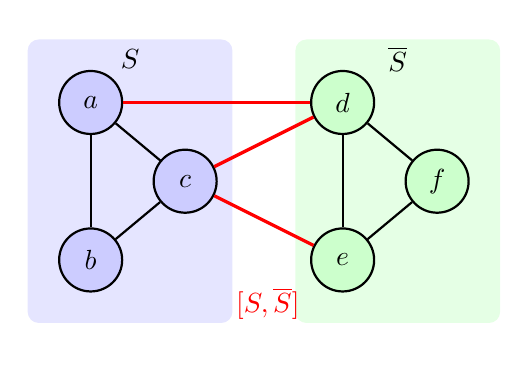
\begin{tikzpicture}[scale=1, every node/.style={circle, draw, thick, minimum size=8mm}]
    \fill[blue!10, rounded corners] (-2.2,-1.8) rectangle (0.4,1.8);
    \fill[green!10, rounded corners] (1.2,-1.8) rectangle (3.8,1.8);

    \node[fill=blue!20] (a) at (-1.4, 1.0) {$a$};
    \node[fill=blue!20] (b) at (-1.4,-1.0) {$b$};
    \node[fill=blue!20] (c) at (-0.2, 0.0) {$c$};

    \node[fill=green!20] (d) at (1.8, 1.0) {$d$};
    \node[fill=green!20] (e) at (1.8,-1.0) {$e$};
    \node[fill=green!20] (f) at (3.0, 0.0) {$f$};

    \draw[thick] (a) -- (b);
    \draw[thick] (a) -- (c);
    \draw[thick] (b) -- (c);
    \draw[thick] (d) -- (e);
    \draw[thick] (d) -- (f);
    \draw[thick] (e) -- (f);

    \draw[very thick, red] (a) -- (d);
    \draw[very thick, red] (c) -- (d);
    \draw[very thick, red] (c) -- (e);

    \node[draw=none, fill=none] at (-0.9, 1.55) {$S$};
    \node[draw=none, fill=none] at (2.5, 1.55) {$\overline{S}$};
    \node[draw=none, fill=none, text=red] at (0.85,-1.55) {$[S,\overline{S}]$};
\end{tikzpicture}
\end{center}

\begin{observation}
    Any minimal disconnecting set of edges will be edge cut, and any edge cut is a disconnecting set of edges. Therefore,
    \[
        \kappa ^{\prime} (G) = \min \left\{ \left\vert \left[ S, \overline{S}  \right] \right\vert  : \varnothing \neq S \subsetneq V  \right\}. 
    \]
\end{observation}

\begin{theorem}[Whitney, 1932] \label{thm: kappa kappa prime delta}
    For any graph \(G\), \(\kappa (G) \le \kappa ^{\prime} (G) \le \delta (G)\).  
\end{theorem}
\begin{proof}
    We first show \(\kappa ^{\prime} (G) \le \delta (G)\): Let \(v\) be a vertex of minimum degree, then removing all its edges isolates it, i.e. 
    \[
        \left\vert \left[ \left\{ v \right\}, V \setminus \left\{ v \right\}   \right]  \right\vert = \deg (v). 
    \]  

    As for \(\kappa (G) \le \kappa ^{\prime} (G)\). Let \(F \subseteq E(G)\) where \(\vert F \vert = \kappa ^{\prime} (G) \) s.t. \(G - F\) is disconnected. Let \(F = [S, \overline{S}]\). If \(\exists x \in S\) and \(y \in \overline{S}\) s.t. \(\left\{ x, y \right\} \notin E(G) \), then for every \(\left\{ u, v \right\} \in [S, \overline{S}] \), if \(u \neq x\), remove \(u\), otherwise remove \(v\). This ensures \(x, y\) are in the remaining graph.  Hence, we can remove \(\le \vert F \vert \) vertices to make remove all edges in \(F\), and at the end, \(x, y\) are disconnected. Hence, \(\kappa (G) \le \vert F \vert = \kappa ^{\prime} (G) \). Otherwise, if \(\left\{ x, y \right\} \in E(G) \) for all \(x \in S\) and \(y \in \overline{S}\), then
    \[
        \vert F \vert = \vert S \vert \cdot \vert \overline{S} \vert = \vert S \vert \cdot (n - \vert S \vert ) \ge n - 1. 
    \]                
    Hence, \(\kappa (G) \le n - 1 \le \vert F \vert = \kappa ^{\prime} (G) \). 
\end{proof}

\begin{exercise}[HW]
    \(\forall k \le \ell \le m\), \(\exists \) a graph \(G\) with 
    \[
        \kappa (G) = k, \quad \kappa ^{\prime} (G) = \ell, \quad \delta (G) = m. 
    \]  
\end{exercise}

\begin{question}
    "Is \(G\) \(k\)-connected?" is a decision problem of P or NP or co-NP?  
\end{question}

\begin{answer}
    It is co-NP since we can verify a disconnected set of size \(< k\) in polynomial time. Also, if \(k\) is a constant, then we can check if all \(\binom{n}{k-1}\) vertex subsets are not disconnecting sets in polynomial time by brute forces.      
\end{answer}

\paragraph{Characterization of \(k\)-connected graphs}
If \(k = 2\), then it means we can remove any vertex from the graph and the graph remains connected. Hence, we have a sufficient condition for 2-connectivity: For any two vertices \(u, v\), there are two internally vertex disjoint \(uv\)-path, i.e. two \(uv\)-path with only \(u, v\) are common vertices of 2 paths. 

\begin{center}
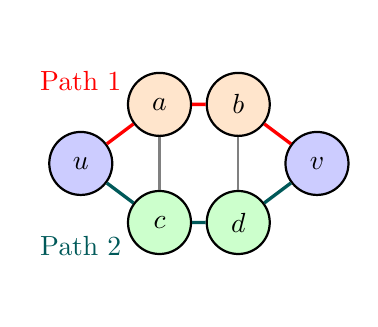
\begin{tikzpicture}[scale=0.5, every node/.style={circle, draw, thick, minimum size=8mm}]
    \node[fill=blue!20] (u) at (0,0) {$u$};
    \node[fill=blue!20] (v) at (6,0) {$v$};

    \node[fill=orange!20] (a) at (2,1.5) {$a$};
    \node[fill=orange!20] (b) at (4,1.5) {$b$};

    \node[fill=green!20] (c) at (2,-1.5) {$c$};
    \node[fill=green!20] (d) at (4,-1.5) {$d$};

    % top path
    \draw[very thick, red] (u) -- (a) -- (b) -- (v);

    % bottom path
    \draw[very thick, teal!70!black] (u) -- (c) -- (d) -- (v);

    % optional extra edges to suggest a larger graph
    \draw[thick, gray] (a) -- (c);
    \draw[thick, gray] (b) -- (d);

    \node[draw=none, fill=none, text=red] at (0,2.1) {Path 1};
    \node[draw=none, fill=none, text=teal!70!black] at (0,-2.1) {Path 2};
\end{tikzpicture}
\end{center}

\begin{theorem}[Whitney, 1932]
    A graph is \(2\)-connected if and only if for every \(u, v \in V(G)\), there are two internally disjoint \(uv\)-paths.   
\end{theorem}

\begin{proof}
\hfill
     \begin{itemize}
        \item [\((\impliedby )\)] Consider \(G - x\) for any \(x \in V\), then for any \(u, v \neq x\), we have two internally disjoint \(uv\)-path, where \(x\) is in at most one if them. Hence, the path without \(x\) is in \(G - x\), which means \(G - x\) is connected, i.e. \(G\) is 2-connected.
        \item [\((\implies)\)] We do induction on \(d_G(u, v)\). For the base case: \(d_G(u, v) = 1\), then since \(2\)-connected implies \(2\)-edge-connected by \autoref{thm: kappa kappa prime delta}, so \(G - \left\{ u, v \right\} \) is connected. Hence, there is a \(uv\)-path \(P\) in \(G - \left\{ u, v \right\} \). Thus, \(\left\{ u, v \right\} \) and \(P\) are two internally disjoint \(uv\)-path. Now we do the induction step: Let \(d_G(u, v) \ge 2\). Let \(Q\) be a shortest \(uv\)-path. Let \(x\) be the vertex preceding \(v\) on \(Q\), then \(d_G(u, x) = d_G(u, v) - 1\). By induction hypothesis, there are two internally-disjoint \(ux\)-paths in \(G\), say \(P_1, P_2\). Since \(G\) is 2-connected, \(G - \left\{ x \right\} \) is connected, so there is a \(uv\)-path in \(Q^{\prime}\) in \(G - \left\{ x \right\} \). Starting from \(v\), trace back along \(Q^{\prime} \) until the first meet with \(P_1 \cup P_2\), switch to that path and go back to \(u\). Using the other path, go from \(u\) to \(x\), and use the edge from \(x\) to \(v\). Hence, we have two internally disjoint \(uv\)-paths.                            
        \begin{center}
        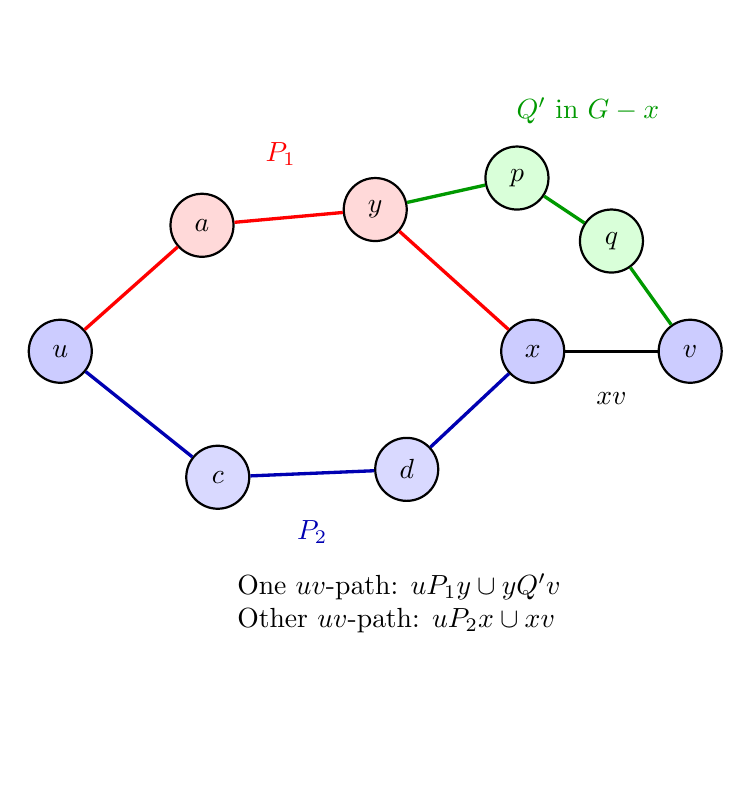
\begin{tikzpicture}[scale=1.0, every node/.style={circle, draw, thick, minimum size=8mm}]
            \node[fill=blue!20] (u) at (0,0) {$u$};
            \node[fill=blue!20] (x) at (6,0) {$x$};
            \node[fill=blue!20] (v) at (8,0) {$v$};

            \node[fill=red!15] (a) at (1.8,1.6) {$a$};
            \node[fill=red!15] (y) at (4.0,1.8) {$y$};

            \node[fill=blue!15] (c) at (2.0,-1.6) {$c$};
            \node[fill=blue!15] (d) at (4.4,-1.5) {$d$};

            \node[fill=green!15] (p) at (5.8,2.2) {$p$};
            \node[fill=green!15] (q) at (7.0,1.4) {$q$};

            % P1 and P2
            \draw[very thick, red] (u) -- (a) -- (y) -- (x);
            \draw[very thick, blue!70!black] (u) -- (c) -- (d) -- (x);

            % Q'
            \draw[very thick, green!60!black] (y) -- (p) -- (q) -- (v);

            % edge xv
            \draw[very thick] (x) -- (v);

            % labels
            \node[draw=none, fill=none, text=red] at (2.8,2.5) {$P_1$};
            \node[draw=none, fill=none, text=blue!70!black] at (3.2,-2.3) {$P_2$};
            \node[draw=none, fill=none, text=green!60!black] at (6.7,3.05) {$Q'$ in $G-x$};
            \node[draw=none, fill=none] at (7.0,-0.6) {$xv$};

            % guide text
            \node[draw=none, fill=none, align=left] at (4.3,-3.2)
            {One $uv$-path: $uP_1y \cup yQ'v$\\Other $uv$-path: $uP_2x \cup xv$};
        \end{tikzpicture}
        \end{center}
     \end{itemize} 
\end{proof}

\begin{theorem}
    A graph \(G\) is \(2\)-connected if and only if \(\delta (G) \ge 1\) and for any two edges in the graph, there is a cycle combining both.   
\end{theorem}
\begin{proof}
    We first give a lemma:
    \begin{lemma}[Extension Lemma]
        If \(G\) is \(k\)-connected, and \(G^{\prime}\) is obtained by adding a vertex \(v\) of degree \(\ge k\) to \(G\), then \(G^{\prime} \) is \(k\)-connected.        
    \end{lemma}

    \begin{proof}
        Let \(S \subseteq V (G^{\prime})\) and \(\vert S \vert \le k - 1\), then we need to show that \(G^{\prime} - S\) is connected. If \(v \in S\), then \(G^{\prime} - S = G - S\), which is connected since \(G\) is \(k\)-connected. If \(S \subseteq V(G)\), then \(G - S\) is connected since \(G\) is \(k\)-connected. Since \(v\) has \(\ge k\) neighbors, and \(\vert S \vert \le k - 1 \), so \(v\) still has a neighbor in \(G - S\), which shows \(G^{\prime} - S\) is connected.               
    \end{proof}

    Now we prove the theorem.

    \begin{itemize}
        \item [\((\impliedby)\)] Given \(u, v \in V(G)\), let \(e, f\) be edges containing \(u, v\), respectively. Since \(e, f\) are on a cycle containing \(u, v\), so there are two internally disjoint \(uv\)-path, i.e. \(G\) is 2-connected. 
        \item [\((\implies)\)] Let \(G\) be 2-connected, and \(e, f \in E(G)\). Let \(G^{\prime}\) be obtained by adding a vertex \(u\) to the endpoints of \(e\) to \(G\). Then by the extension lemma, \(G^{\prime}\) is \(2\)-connected. Now let \(G^{\prime\prime}\) be obtained by adding a vertex \(v\) adjacent to endpoints of \(f\) to \(G^{\prime}\), then \(G^{\prime\prime} \) is \(2\)-connected by extension lemma. By Whitney, there exists internally disjoint paths \(P_1, P_2\) from \(u\) to \(v\). Consider \(P_1 \cup P_2\), replacing \(x-u-y\) by \(\left\{ x, y \right\} = e \) and \(x^{\prime} - v - y^{\prime}\) with \(\left\{ x^{\prime} , y^{\prime}  \right\} = f \), we get a cycle in \(G\) containing \(e\) and \(f\). 
        
        \begin{center}
            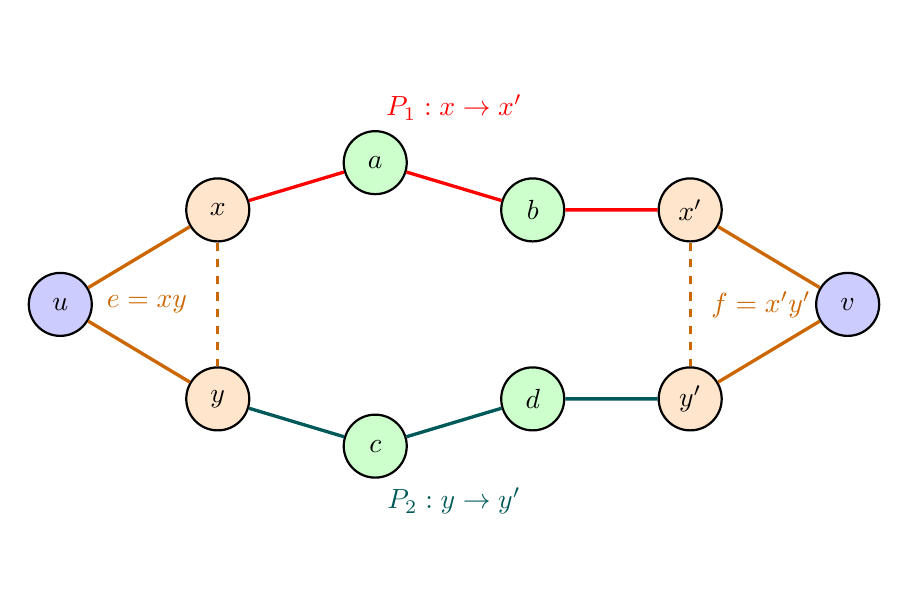
\begin{tikzpicture}[scale=1.0, every node/.style={circle, draw, thick, minimum size=8mm}]
                % left gadget for e
                \node[fill=blue!20] (u) at (0,0) {$u$};
                \node[fill=orange!20] (x) at (2.0,1.2) {$x$};
                \node[fill=orange!20] (y) at (2.0,-1.2) {$y$};

                % middle vertices on the two uv-paths
                \node[fill=green!20] (a) at (4.0,1.8) {$a$};
                \node[fill=green!20] (b) at (6.0,1.2) {$b$};
                \node[fill=green!20] (c) at (4.0,-1.8) {$c$};
                \node[fill=green!20] (d) at (6.0,-1.2) {$d$};

                % right gadget for f
                \node[fill=orange!20] (xp) at (8.0,1.2) {$x'$};
                \node[fill=orange!20] (yp) at (8.0,-1.2) {$y'$};
                \node[fill=blue!20] (v) at (10.0,0) {$v$};

                % edges from u and v to chosen edge endpoints
                \draw[very thick, orange!80!black] (u) -- (x);
                \draw[very thick, orange!80!black] (u) -- (y);
                \draw[very thick, orange!80!black] (xp) -- (v);
                \draw[very thick, orange!80!black] (yp) -- (v);

                % two internally disjoint uv paths
                \draw[very thick, red] (x) -- (a) -- (b) -- (xp);
                \draw[very thick, teal!70!black] (y) -- (c) -- (d) -- (yp);

                % original edges in G
                \draw[very thick, dashed, orange!80!black] (x) -- (y);
                \draw[very thick, dashed, orange!80!black] (xp) -- (yp);

                % labels
                \node[draw=none, fill=none, text=orange!80!black] at (1.1,0) {$e=xy$};
                \node[draw=none, fill=none, text=orange!80!black] at (8.9,0) {$f=x'y'$};
                \node[draw=none, fill=none, text=red] at (5.0,2.5) {$P_1: x\to x'$};
                \node[draw=none, fill=none, text=teal!70!black] at (5.0,-2.5) {$P_2: y\to y'$};
            \end{tikzpicture}
        \end{center}
    \end{itemize}       
\end{proof}

\begin{corollary}
    2-connectivity problem is in NP \(\cap \) co-NP. 
\end{corollary}

\begin{theorem}[Global vertex Menger]
    \(G\) is \(k\)-connected if and only if for any \(u, v \in V(G)\), \(\exists \) \(k\) internally-disjoint \(uv\)-path.       
\end{theorem}

\begin{proof}
    \hfill 
    \begin{itemize}
        \item [\((\impliedby)\)] Obvious. 
        \item [\((\implies )\)] Harder.
    \end{itemize}

    \begin{remark}
        This shows \(k\)-connectivity is in NP \(\cap \) co-NP.  
    \end{remark}

    \begin{remark}
        However, it is really hard to prove the "harder" direction directly. Instead, we use Local vertex Menger to prove this theorem.
    \end{remark}
\end{proof}

\begin{definition}
    Given \(G = (V, E)\), \(u, v \in V\). Then,
    \begin{align*}
        \kappa (u, v) &= \min \left\{ \vert S \vert: S \subseteq V \setminus \left\{ u, v \right\} \text{ and } \nexists uv\text{-path in } G - S \ (S \text{ is a } uv \text{-separator})    \right\}   \\
        \lambda (u, v) &= \max \left\{ \vert P \vert: P \text{ is a collection of internally disjoint } uv\text{-path}    \right\}.  
    \end{align*}  
\end{definition}

\begin{theorem}[Local vertex Menger]
    If \(G = (V, E)\) is a graph, and \(u, v \in V\) with \(\left\{ u, v \right\} \notin E \), then \(\kappa (u, v) = \lambda (u, v)\).    
\end{theorem}

\begin{claim}
        Local vertex Menger implies Global vertex Menger.
    \end{claim}
    \begin{explanation}
        Let \(G\) be \(k\)-connected, \(u, v \in V(G)\). If \(\left\{ u, v \right\} \notin E(G) \), then Local vertex Menger implies \(\lambda (u, v) = \kappa (u, v) \ge \kappa (G) \ge k\). Hence, we have \(k\) internally disjoint \(uv\)-paths, which is what global vertex Menger states. 

        If \(\left\{ u, v \right\} \in E(G) \): Let \(G^{\prime} \equiv  G - \left\{ u, v \right\} \), so \(\kappa (G^{\prime} ) \ge \kappa (G) - 1\). Apply local vertex Menger to \(G^{\prime} \):
        \[
            \lambda _{G^{\prime} }(u, v) = \kappa_{G^{\prime} }(u, v) \ge \kappa (G^{\prime} ) \ge \kappa (G) - 1 \ge k - 1.
        \]         
        Hence, in \(G^{\prime}\), there are \(k - 1\) internally disjoint \(uv\)-paths, and in \(G\) we have these \(k - 1\) paths and \(\left\{ u, v \right\} \), so we have \(k\) internally disjoint \(uv\)-paths in \(G\), and we're done.        
    \end{explanation}